\documentclass{article}
\usepackage[a4paper,left=3.5cm,right=2.5cm,top=2.5cm,bottom=2.5cm]{geometry}
%%\usepackage[MeX]{polski}
%%\usepackage[cp1250]{inputenc}
\usepackage{polski}
\usepackage[utf8]{inputenc}
\usepackage[pdftex]{hyperref}
\usepackage{makeidx}
\usepackage[tableposition=top]{caption}
\usepackage{algorithmic}
\usepackage{graphicx}
\usepackage{enumerate}
\usepackage{multirow}
\usepackage{amsmath} %pakiet matematyczny
\usepackage{amssymb} %pakiet dodatkowych symboli
%opening
\title{Cabanells}
\author{Karolina Ścibek}

\begin{document}
\maketitle

\section{Cabanells}
,,Hiszpańska gmina w Katalonii'', w prowincji Girona,w comarce Alt Empordà.
Powierzchnia gminy wynosi $4,48km^2$. Zgodnie z danymi INE, w $2005$ roku liczba ludności wynosiła $249$, a gęstość zaludnienia $55,62$ $osoby/\ km^2$. Wysokość bezwzględna gminy równa jest $194$ metry.
\begin{figure}[h!]
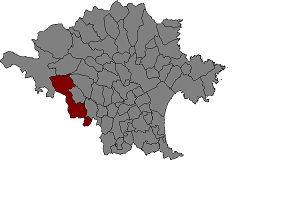
\includegraphics[width=0.5\textwidth]{mapacabanelles.jpg}
\caption{Położenie gminy na mapie comarki Alt Empordà.}
\centering
\end{figure}


\section{Miejscowości}
W skład gminy Cabanelles wchodzi sześć miejscowości, w tym miejscowość gminna o tej samej nazwie:Cabanelles – liczba ludności: $80$
Espinavessa – $72$
L'Estela –$ 3$
Queixàs – $54$
Sant Martí Sesserres – $7$
Vilademires – $33$

\begin{table}[here]
\centering \caption{\ Demografia }
\begin{tabular}{cccccc}
$1991$ & $1996$ &  $2001$ &$2004$ & $2005$ & $2006$\\
\hline
$232$ & $227$ & $225$ & $244$ & $249$ & $240$\\
\end{tabular}
\end{table}






 


\end{document}